\section{Effect of Bond Market Participation}

\subsection{Correlation of implied and observed rates}
Next, I follow the same framework in computing Euler equation implied interest rates for both bondholders and nonbondholders. I estimate two VARs using the time series aggregated from the two groups as described in \autoref{cex-data}, using CEX data from 1996:I to 2012:IV (68 quarters). As before, I set the discount factor $\beta$ to be 0.9926.

In this section, I only compute implied interest rates using CRRA utility --- that is, $\phi = 0$ and $\nu = 1$. The four utility specifications I evaluated in the previous section produced results that were qualitatively very similar: positive correlations between implied and observed rates, but spreads negatively correlated with the stance of monetary policy. I choose to single out CRRA utility (SEP) because it is the simplest model, which nonetheless gives the least negative FFR coefficient in the spread regression (see \autoref{nipa-spread}). This suggests that among the four utility models, the spread between observed and implied rates is least systematically related to monetary policy under the assumption of CRRA utility.

\begin{figure}[b]
\centering
\captionsetup{singlelinecheck=false, justification=centering}
\begin{tabular}{ccc}
NIPA & CEX Bondholders & CEX Nonbondholders \\
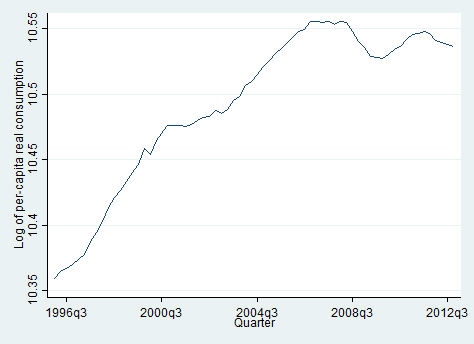
\includegraphics[width=0.31\textwidth]{figs/nipa/log_consumption} &
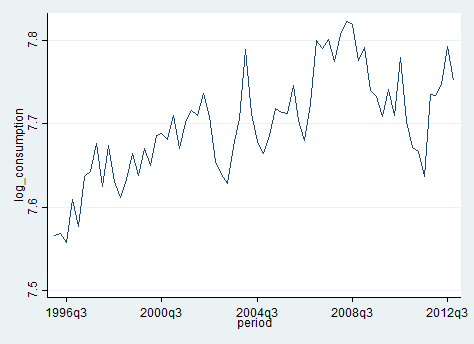
\includegraphics[width=0.31\textwidth]{figs/cex/log_consumption_bh} &
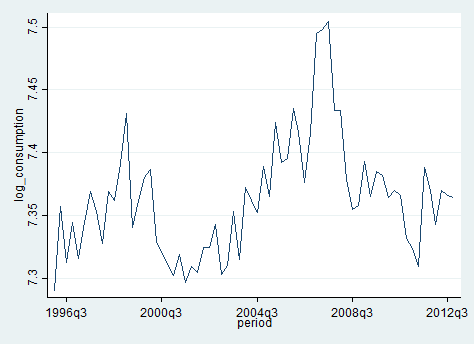
\includegraphics[width=0.31\textwidth]{figs/cex/log_consumption_nbh}
\end{tabular}
\caption{Comparison of log of real consumption $c_t$ from 1996:I to 2012:IV}
\label{log_consumption_series}
\end{figure}

I set the coefficient of relative risk aversion $\alpha$ to be 0.2, in contrast to the previous section, as well as both \cite{canzoneri07} and \cite{collard11}, where $\alpha = 2$. The consumption, income, and leisure paths that I aggregate from household-level CEX data are much more volatile than the nationwide aggregates from NIPA that I use in the replication. In \autoref{log_consumption_series}, I compare the log of real consumption $c_t$ generated from NIPA to those of CEX bondholders and nonbondholders. The paths of the other series (leisure fraction, log of real disposable income, and log of output less consumption) are similarly more volatile when aggregated from household-level data.

\begin{table}[b!]
\centering
\caption{Summary statistics for nominal and real rates (annualized rates)}
\label{implied-vs-ffr-cex}
\begin{tabular}{lccc} \hline
& Data & CEX Bondholders & CEX Nonbondholders \\ \hline
\multicolumn{4}{c}{Real interest rates} \\ \hline
\csvreader[head to column names, late after line = \\]%
  {tables/cex/real.csv}{}%
  {\stat & \data & \cexbh & \cexnbh} \hline
\multicolumn{4}{c}{Nominal interest rates} \\ \hline
\csvreader[head to column names, late after line = \\]%
  {tables/cex/nominal.csv}{}%
  {\stat & \data & \cexbh & \cexnbh} \hline
\end{tabular}
\end{table}

I argued previously that the Euler equation implied rate is proportional to expected consumption growth. From \eqref{nominal-euler-crra}, it also increases in the risk aversion coefficient $\alpha$: $$\frac{1}{1 + i_t} = \beta \exp \paren{ -\alpha \bracket{ \E_t c_{t+1} - c_t } - \E_t \pi_{t+1} + \mathrm{constant\ terms} }$$
In order to achieve implied interest rates approximately in the range we see in real life, a much lower risk aversion is needed to offset the large consumption growth fluctuations in the aggregated CEX data. (Net consumption growth is approximately $\log \paren{\frac{C_t}{C_{t-1}}} = c_t - c_{t-1}$.) Since the CEX consumption growth fluctuations are about ten times larger than those seen in the NIPA data in the same time span, I choose $\alpha$ to be ten times smaller than in the previous section, giving $\alpha = 0.2$.

% TODO: In the appendix, I also report results for $\alpha = 2$, 1, and 0.5.

In \autoref{implied-vs-ffr-cex}, I report summary statistics for the interest rates implied by the consumption, income, and leisure paths of bondholders and nonbondholders. As in the aggregate analysis, the standard deviations of the implied rates are similar to those seen in the data, while the levels are higher overall. The correlation between implied and ex post rates is higher in both the real and nominal cases for bondholders (0.235 and 0.193 respectively) than for nonbondholders (0.133 and 0.028). This could suggest that bondholders --- households who actually have a position in the bond market --- are more likely to adjust their consumption paths in response to changes in the interest rate than are nonbondholders. If this were the case, the interest rates implied by their consumption paths would more resemble observed rates.

\begin{table}[b]
\centering
\caption{Test of difference in correlations between bondholders and nonbondholders}
\label{cex-correlation-test}
\begin{tabular}{lcccc} \hline
& $\rho_{_{BH}}$ & $\rho_{_{NBH}}$ & $\rho_{_{BH}}' - \rho_{_{NBH}}'$ & SE \\ \hline
Real interest rates    & 0.235 & 0.133 & 0.106 & 0.180 \\
Nominal interest rates & 0.193 & 0.028 & 0.168 & 0.180 \\ \hline
\end{tabular}
\end{table}

To test whether the correlation is significantly higher for bondholders than for nonbondholders, I use Fisher's transformation. First, I transform each correlation $\rho$ by $$\rho' = \frac{1}{2} \log \paren{\frac{1+\rho}{1-\rho}}$$
Then the difference between the transformed correlations, $\rho_{_{BH}}' - \rho_{_{NBH}}'$, is normally distributed with standard error $\sqrt{\frac{1}{n_{_{BH}} - 3} + \frac{1}{n_{_{NBH}} - 3}}$. I report these estimates in \autoref{cex-correlation-test}. The difference between correlations for bondholders and nonbondholders is not significant for both real and nominal interest rates.

\begin{figure}[h!]
\ContinuedFloat*
\centering
\begin{tabular}{cc}
Bondholders ($\rho = 0.235$) & Nonbondholders ($\rho = 0.133$) \\
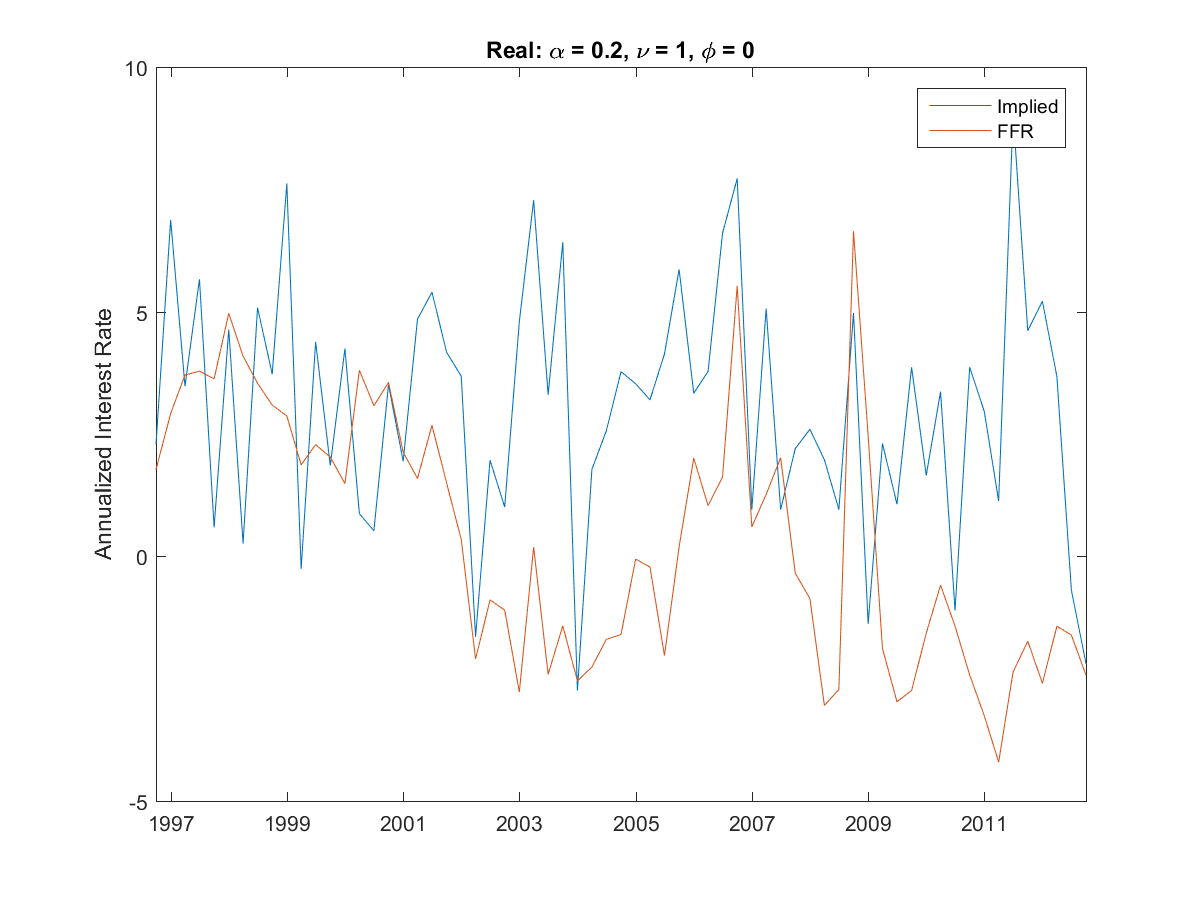
\includegraphics[width=0.49\textwidth]{figs/cex/implied-vs-ffr/bh_real} &
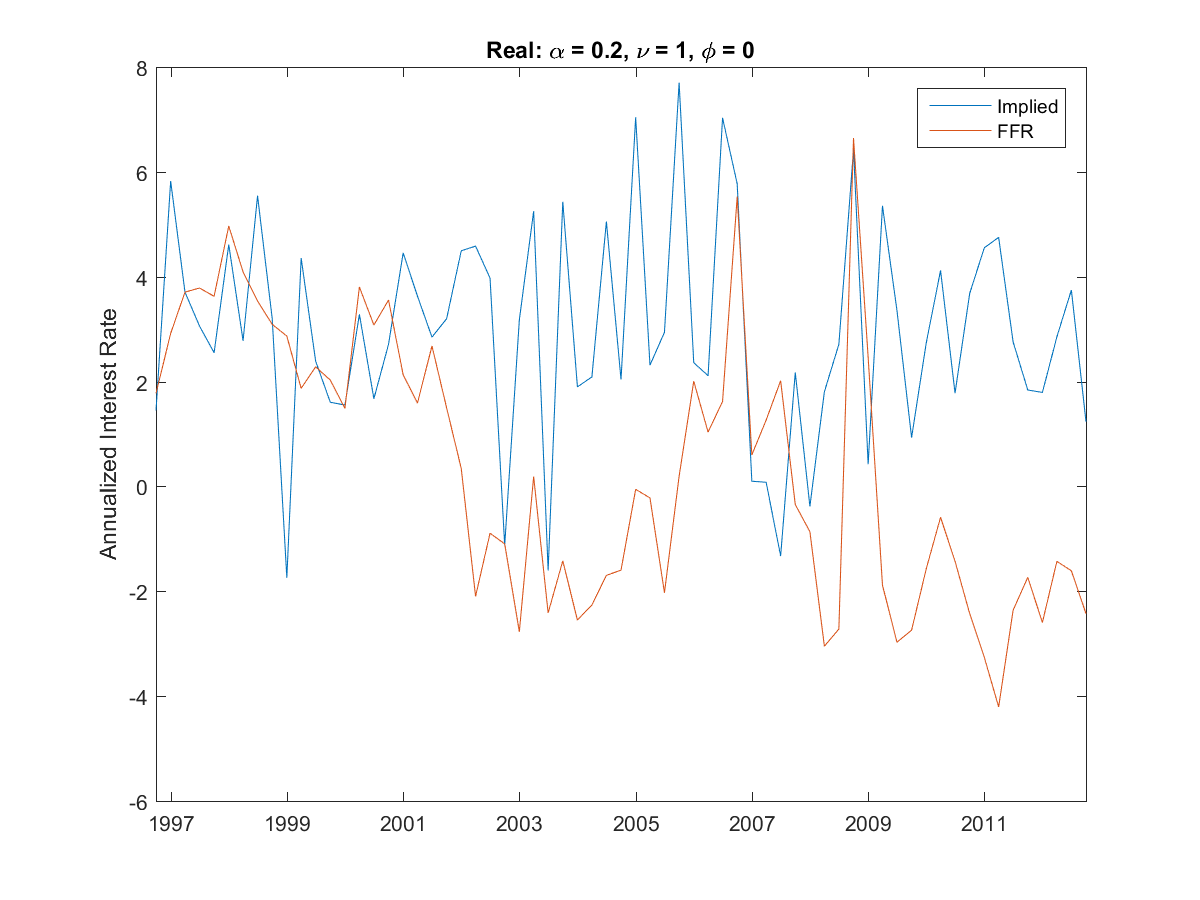
\includegraphics[width=0.49\textwidth]{figs/cex/implied-vs-ffr/nbh_real}
\end{tabular}
\caption{Implied vs. observed real rates}
\label{implied-vs-ffr-cex-real}
\end{figure}

\begin{figure}[h!]
\ContinuedFloat
\centering
\begin{tabular}{cc}
Bondholders ($\rho = 0.193$) & Nonbondholders ($\rho = 0.028$) \\
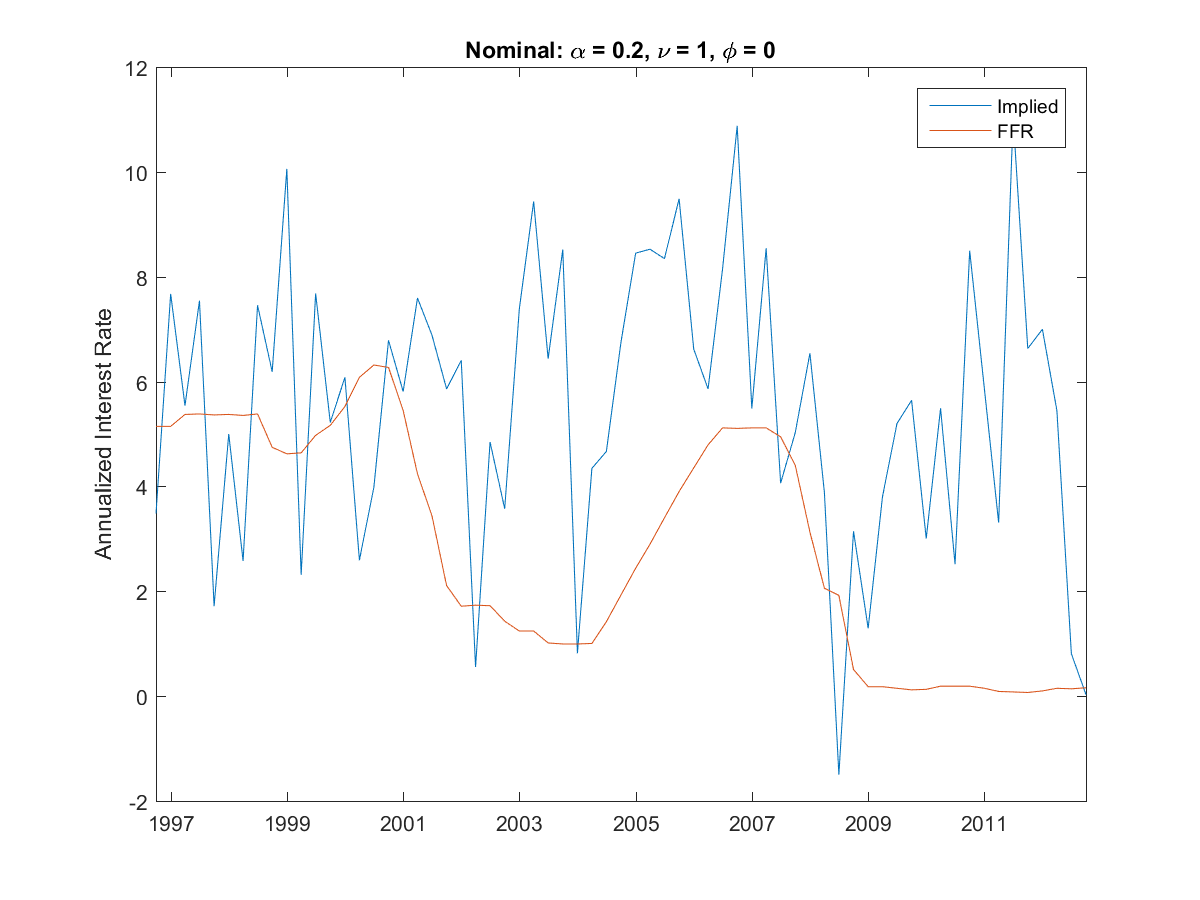
\includegraphics[width=0.49\textwidth]{figs/cex/implied-vs-ffr/bh_nominal} &
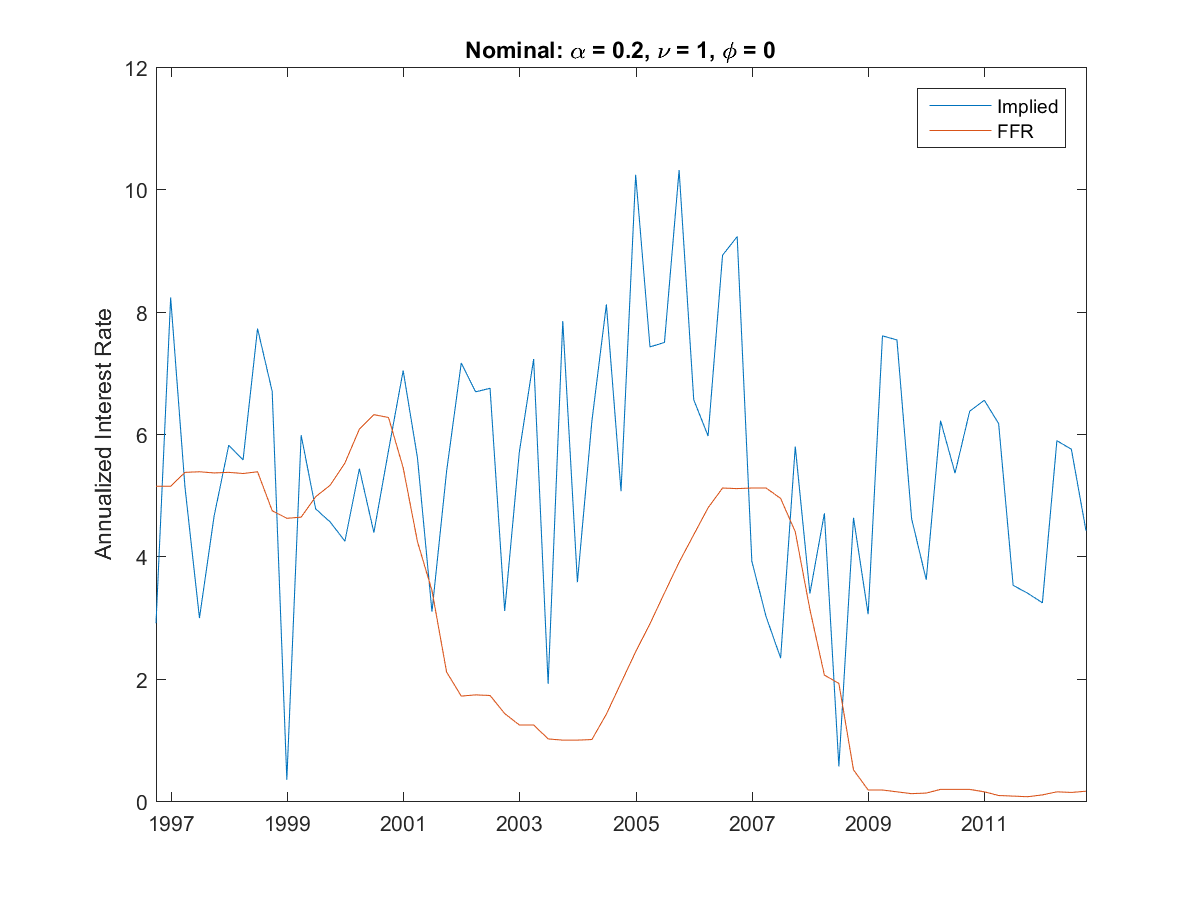
\includegraphics[width=0.49\textwidth]{figs/cex/implied-vs-ffr/nbh_nominal}
\end{tabular}
\caption{Implied vs. observed nominal rates}
\label{implied-vs-ffr-cex-nominal}
\end{figure}

Comparing the interest rate paths qualitatively in \autoref{implied-vs-ffr-cex-real} and \autoref{implied-vs-ffr-cex-nominal} shows how noisy the implied rates are in this specification. The risk aversion coefficient $\alpha = 0.2$ implies an elasticity of intertemporal substitution of $\frac{1}{\alpha} = 5$, which is extremely high and well outside the range of estimated elasticities. \cite{guvenen06} cites elasticity values in the literature in the range of 1 for stockholders and 0.1 for nonstockholders. This suggests that the volatility of the consumption paths aggregated from the CEX is mostly the result of the small sample size and is not necessarily representative of the actual variation in households' consumption choices.



\subsection{Response of spread to monetary policy}
So much for the correlations between the implied and observed rates. Since I argued that the correlation is not necessarily the most reliable indicator of fit, it is reasonable to again check how the spread between implied and observed rates depends on the stance of monetary policy. To test whether the FFR coefficient on spread is significantly different for bondholders and nonbondholders, I estimate the linear model
\begin{equation}
\label{spread-ffr-bondholder-regression}
\mathrm{spread}_t = b_0 + b_1 \mathrm{FFR}_t + b_2 \mathrm{bondholder} + b_3 \mathrm{bondholder} \times \mathrm{FFR}_t + \sum_{j=1}^4 a_j \mathrm{spread}_{t-j}
\end{equation}
The estimated coefficients and standard errors for the non-lag terms are reported in \autoref{cex-spread-regression}. The FFR coefficients for real spreads are $b_1 = -1.063$ for nonbondholders and $b_1 + b_3 = -0.930$ for bondholders; for nominal spreads they are -0.396 for nonbondholders and -0.398 for nonbondholders. The difference in slopes $b_3$ is not significant for either real or nominal spreads.

\begin{table}[b]
\centering
\caption{Response of spread to FFR for bondholders and nonbondholders}
\label{cex-spread-regression}
\begin{tabular}{lccc} \hline
& FFR & Bondholder & Bondholder $\times$ FFR \\ \hline
\multicolumn{4}{c}{Real spreads} \\ \hline
Coef & -1.063  & 0.105   & 0.133 \\
SE   & (0.144) & (0.408) & (0.157) \\ \hline
\multicolumn{4}{c}{Nominal spreads} \\ \hline
Coef & -0.396  & -0.002  & -0.123 \\
SE   & (0.153) & (0.463) & (0.178) \\ \hline
\end{tabular}
\end{table}

As in the aggregate analysis, the negative FFR coefficients themselves are significant at below the 1 percent level. This is further evidence that the consumption Euler equation (in the form that I have examined) does not adequately describe the relationship between expected consumption growth and the interest rate. Separating out bondholders, who are perhaps most likely to optimize according to the Euler equation, does not improve the negative relationship between the spread and the federal funds rate.